\chapter{Related Work} 
\label{ch:relatedwork}

As the field of AI has grown, more and more researchers are looking into the extent of the capabilities of AI.  The creation of music with computers has gained increased attention within the last decade, however, this does not mean that these tools have gained popularity among users.  Quite a few of these composers that have been developed, but only a very small number of them have seen industry use and almost none of them have been used outside of research or these niche areas in industry.

\vspace{\baselineskip}

The reason for this primarily is that the focus of researchers when creating these tools is how advanced the composer can be and what new ways can AI be employed to create more original music.  Their focus is not at all on how these tools can be made it a way that they might find a larger user base or even a user base at all.  This limits what might come of these technologies now and in the future.

\vspace{\baselineskip}

Setting this aside, however, the researchers that have developed these composers have created some very impressive tools capable of creating very convincing music.  This project aims more to guide the user through the process of composing music which is different than majority of the research projects in this area that focus on creating a composer that can write its own music, but the writing still contains an important discussion of how computers can be used to create music.

\section{AI Powered Composers}
\label{sec:composers}

The following works discuss several different AI based composers that were created to generate their own music.  For the purpose of this thesis, they will be analyzed for their effectiveness at composing as well as their shortcomings as tools that only have limited usability.  All of these have proven to be effective at creating music, but none of them have shown popularity as music composition tools.

\subsection{FlowComposer}
\label{subsec:flowcomposer}

Of the existing AI composers, FlowComposer is the only one that has seen use in industry \cite{Papadopoulos_2016}.  An album that was recorded consisting of only music created with FlowComposer was released in 2017 \cite{Papadopoulos_2016}.  This is also one of the only tools that has an actual visual user interface and is not strictly accessed through the command line.  It is currently being developed as part of Sony CSL and Flow Machines, but is not available to the public for use \cite{Papadopoulos_2016}.  An audio example of what FlowComposer is capable of producing is available on their website, but access to the tool itself is not provided \cite{Flow_2018}.

\vspace{\baselineskip}

FlowComposer was designed to create new songs automatically in any style or can generate the style based on user provided parameters and input \cite{Papadopoulos_2016}.  This tool is capable of re-harmonization (taking an existing melody and create new harmonies in different styles), variation (taking the melody and introducing variations into the pitch content and rhythm), and rendering (playing back a given score as if it were being performed) \cite{Flow_2018}.

\vspace{\baselineskip}

The musical output of this tool is a lead sheet that is scored for a full band.  The music that FlowComposer produces fits into the category of popular songs (e.g. Pop, Jazz, Rock, R \& B, etc.).  It comes out fully notated and able to be performed or recorded.  It is a very high quality tool and very capable at writing songs, but due to its research based nature, is kept from the public.  It is highly likely also that this tool would be very expensive if it were available to the public.  Maybe in the future, this will be a tool that is made available, but it will doubtfully ever be accessible to the average person due to the potential price.

\subsection{BachProp}
\label{subsec:bachprop}

BachProp is a neural composer algorithm that was created to be able to compose new music in any style \cite{Colombo_2018Com}.  It was trained initially on the chorales of J. S. Bach, but is able to compose in any style when given appropriate training data \cite{Colombo_2018Com}.  The data is fed to the composer through MIDI files which are mathematically normalized before being translated into probability data that the algorithm uses to predict melodic direction and shape \cite{Colombo_2018Com}.  For the evaluation of BachProp, audiences were asked to rate several string quartets that it composed after it was trained on string quartets by Haydn and Mozart \cite{Colombo_2018Com}.  Based on the results of the surveys, the music was not only well received, but it was also quite convincingly in the appropriate style and character \cite{Colombo_2018Com}.

\vspace{\baselineskip}

The process of actually performing crowd based musical validation is quite important here.  Rather than the researchers who developed the composer rating the music, they had general audiences perform the reviews to better understand the broad appeal of the music.  In this project, a similar crowd based reviewing of the interface was performed.  Participants individually judged their created music in their own terms so that their personal success was measured to be able to determine if the user interface was able to guide them through the composition process.

\vspace{\baselineskip}

BachProp has also been used and evaluated in the composition of music in a number of other styles \cite{Colombo_2018Gen}.  The method of musical representation used by BachProp has proven to be more effective at capturing and later translating the information from the provided training scores than other algorithmic composers \cite{Colombo_2018Gen}.  By normalizing how the musical data is stored, this tool is able to gather and retain more detail from the score than other composers \cite{Colombo_2018Gen}.  This is what makes BachProp more effective at emulating a given style and producing more convincing musical output \cite{Colombo_2018Gen}.

\vspace{\baselineskip}

In order for the several Python libraries that were used to create the composer to cooperate, the musical data for this project was also represented in a normalized manner.  Like BachProp, the data was represented as MIDI events to provide a standard for communication and output.  This also means that at any step in the composition process the data could be imported into any standard music notation program and used externally to the composer as MIDI is the standard for digital music notation representation and playback.

\vspace{\baselineskip}

The largest shortcoming of BachProp is that it was not designed in a way that can be used without extensive music or computer science knowledge.  This means that is highly unlikely that it would ever be picked up by someone who simply wanted to play around with it or experiment with it.  There is an extensive setup involved and it cannot be used by any simple means.  However, BachProp is able to produce high quality music in any style and not just popular music as FlowComposer does.

\subsection{DeepBach}
\label{subsec:deepbach}

DeepBach is a graphical model for musical composition that is designed to be effective at producing polyphonic music in four part hymn format \cite{Hadjeres_2016}.  This is yet another composer that was trained on the music of J. S. Bach in order to teach it the mechanics of composition and in this case, to teach it chorales specifically \cite{Hadjeres_2016}.  This composer is able to produce convincing Bach chorale style pieces that are driven by user parameters and input \cite{Hadjeres_2016}.  The following are examples of output composed by DeepBach.

\begin{figure}[p]
	\centering
	\caption{Scores from Hadjeres's published paper showing DeepBach output \cite{Hadjeres_2016}}
	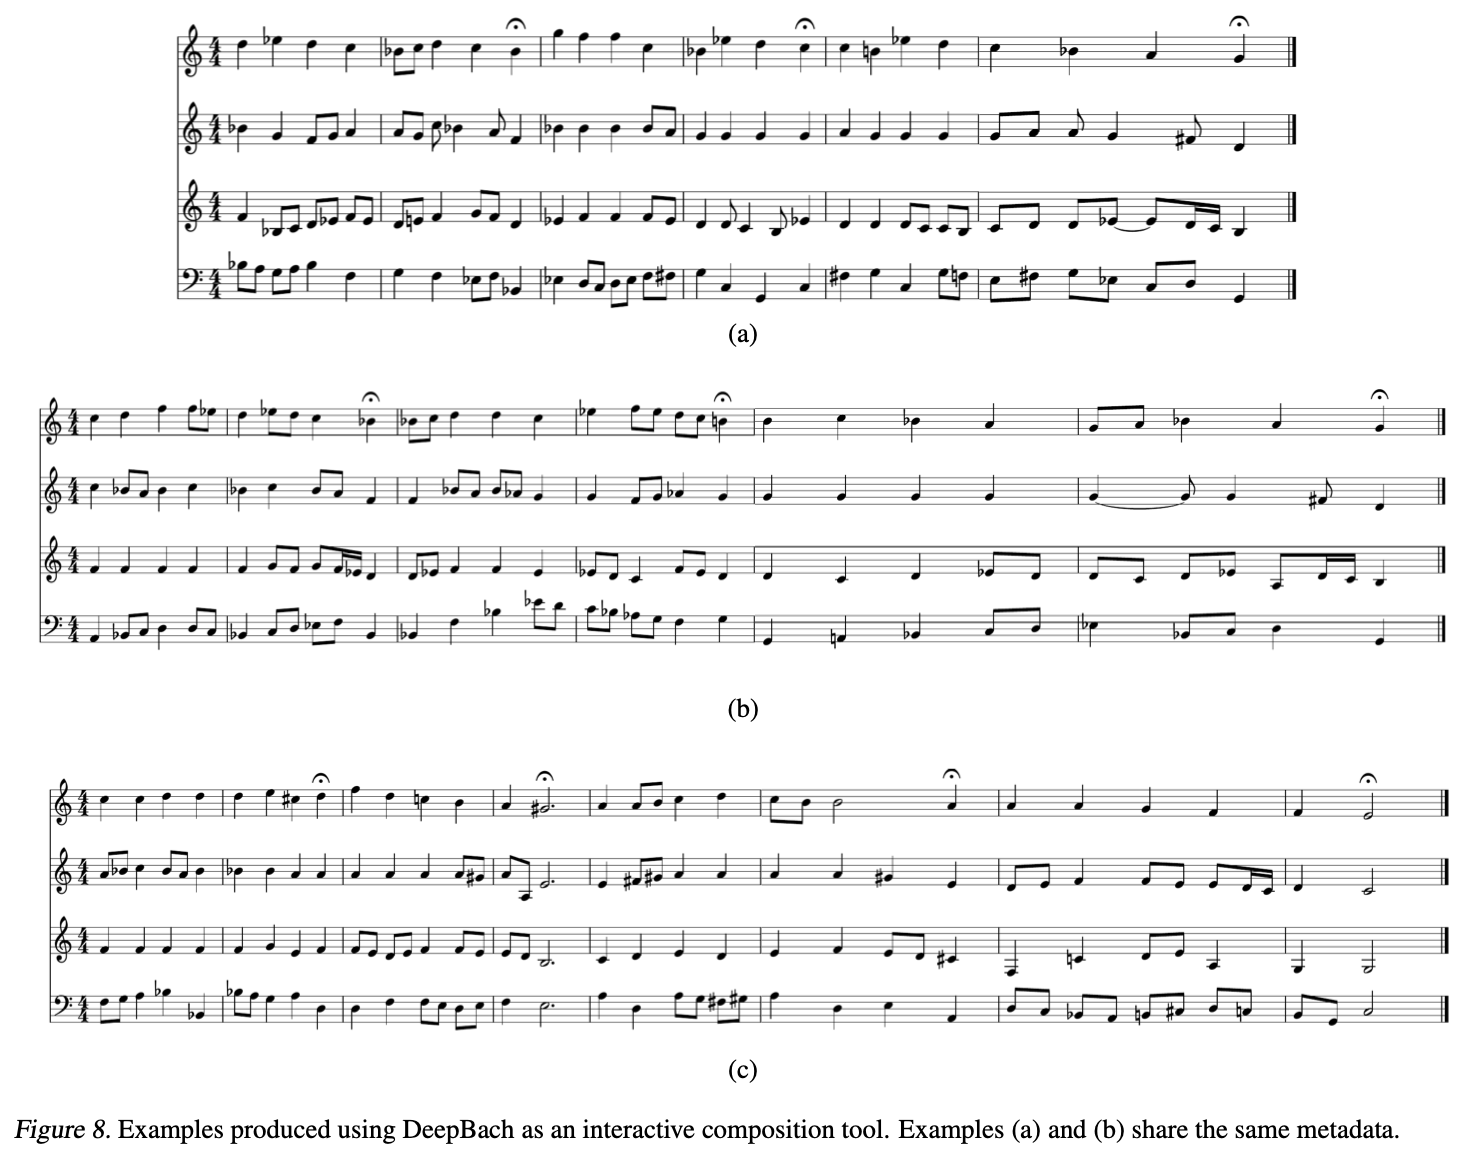
\includegraphics[width=\textwidth]{images/deepbachOutput.png}
\end{figure}

\pagebreak

These scores by DeepBach demonstrate very convincing imitations of Bach chorales.  Upon analysis, the composer has effectively followed the rules of this type of counterpoint as well as captured the style of Bach.  It is important to note that the first two examples share the same user input data and parameters.  This shows that there are at least several different possibilities for harmonization and development of the melodic line.

\vspace{\baselineskip}

DeepBach does provide integration with the notation program MuseScore \cite{Hadjeres_2016}.  This means that there is a way in which people who are familiar with notation software could use this composer.  While this is better than many of the others, it still requires a fair bit of prior knowledge.  Additionally, this composer is not capable of operating in more than four part chorale style.  The potential uses of this composer are very limited due to this fact.